\documentclass[12pt]{article}
\usepackage{fullpage,times}

\usepackage{graphicx}

\makeatletter
\newcommand\TitleSize{\@setfontsize\TitleSize{40}{40}}
\makeatother


\begin{document}                            

%\thispagestyle{empty}

\begin{center}
``Unique games have a tendency to wash up on the Linux shores every so often.
 
{\Large Cultivation is one of the most unique to show up in quite a while.''} 

--PCBurn.com
\end{center}

\vspace{0.5in}

\begin{center}
{\TitleSize Cultivation}


a non-genre video game by Jason Rohrer
\end{center}


Cultivation explores the social interactions within a gardening community.  You lead one family of gardeners, starting with a single individual, and wise choices can keep your genetic line from extinction.  While breeding plants, eating, and mating, your actions impact your neighbors, and the social balance sways between conflict and compromise.  In Cultivation, there is no shooting, but there are plenty of angry looks.

Cultivation features dynamic graphics that are procedurally-generated using genetic representations and cross-breeding.  In other words, game objects are ``grown'' in real-time instead of being hand-painted or hard-coded.  Each plant and gardener in the game is unique in terms of both its appearance and behavior.

In each new game, the fresh behaviors of your new neighbors, combined with the newly-generated  landscape and plants, lead to new challenges.  A strategy that wins one game of Cultivation will not necessarily be effective in the next game.  Thus, even after winning several games, you can never really ``beat'' Cultivation---this sets it apart from most modern video games, which offer a fixed, linear path to victory. 

\vspace{0.25in}

\noindent {\Large Press Photo}

A high-resolution screen shot, suitable for printing, can be downloaded from 
\begin{center}{\bf http://cultivation.sf.net/press/}\end{center}

\vspace{0.125in}

\noindent {\Large Creator Bio}

Jason Rohrer is an independent programmer, scientist, artist, and activist.  He holds two degrees in computer science from Cornell University.  As a peer-to-peer networking developer working in open-source software, he has created several popular programs over the past five years, including MUTE, the first anonymous search-and-download file sharing system.  As of November 2006, MUTE had been downloaded over 850,000 times.  His first video game, Transcend, was included on the Moondance Independent Games compilation.  Cultivation is his second video game project.  A complete list of projects can be found at http://jasonrohrer.n3.net

\vspace{0.25in}

\noindent {\Large Contact Information}
\begin{center}
\begin{tabular}[t]{rl}
Web:  & http://cultivation.sf.net  \\  
Email:  & jcr13@users.sf.net\\
\end{tabular}  
\begin{tabular}[t]{rl}
Phone: &315-265-0585\\ 
Mail:& Jason Rohrer\\ 
&93 Elm St.\\  
&Potsdam, NY 13676\\  
&USA
\end{tabular}
\end{center}

\newpage

\begin{center}

~

\vspace{2in}

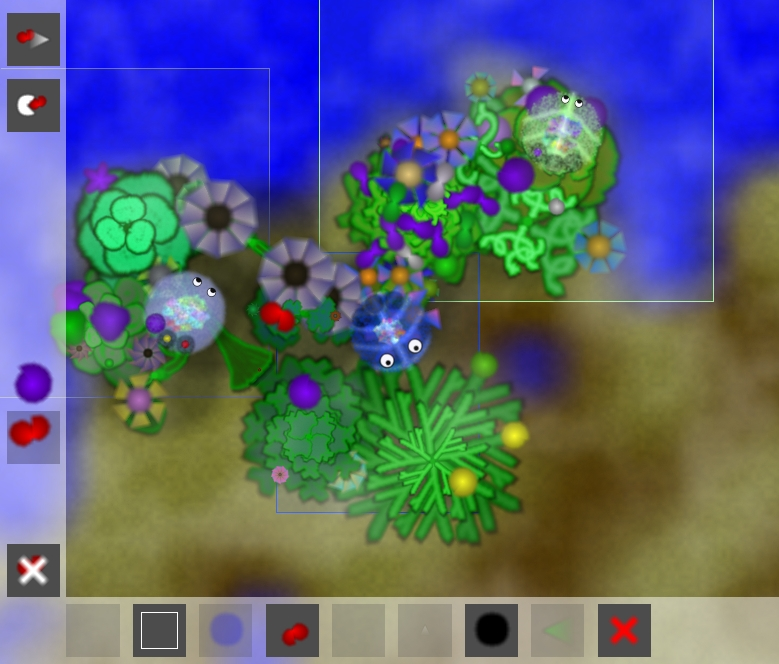
\includegraphics[scale=2]{../../html/press/cultivation.jpg}
\end{center}

\end{document}   
